\section{Anexo 1: Reporte de Estrategia Híbrida de Revisión Bibliográfica}

Para garantizar un marco de antecedentes transparente, exhaustivo y replicable, la selección de la literatura especializada se llevó a cabo mediante una estrategia híbrida basada en la metodología PRISMA 2020. Esta combinó minería de datos bibliográficos en bases científicas de alto impacto con la incorporación sistemática de literatura gris institucional y búsquedas complementarias en repositorios iberoamericanos.

\subsection{Justificación de la Búsqueda y Cadenas de Consulta}
La elección de \textit{Web of Science Core Collection} responde a la necesidad de evaluar la producción académica sometida a rigurosa revisión por pares sobre el bienestar socioeconómico en la región. La consulta fue estructurada en el campo de tema (\textit{Topic}) para vincular las métricas de ingresos y precios con la cobertura geográfica del estudio:

\begin{quote}
\small\ttfamily\raggedright
TS=((("cost of living" OR "purchasing power" OR "household income*" OR "real wage*" OR "minimum wage*" OR "basic food basket*" OR "basic basket*" OR "inflation*" OR "cash transfer*" OR "social transfer*" OR "income distribution" OR "income inequality" OR "informal labor" OR "labor informality") AND ("Chile" OR "Brazil" OR "Brasil" OR "Argentina" OR "Southern Cone" OR "Cono Sur")))
\end{quote}

\subsubsection{Búsqueda Complementaria Regional (SciELO, Redalyc, Dialnet y Google Académico)}
Para mitigar el sesgo de indexación internacional y capturar discusiones empíricas regionales editadas en español y portugués, se ejecutaron cadenas de búsqueda adaptadas en plataformas de acceso abierto:

\begin{itemize}
    \item \textbf{SciELO / Redalyc (Español)}:
    \begin{quote}
    \small\ttfamily\raggedright
    ("costo de vida" OR "poder adquisitivo" OR "ingreso del hogar" OR "salario real" OR "salario mínimo" OR "canasta básica" OR "inflación" OR "transferencias monetarias" OR "desigualdad de ingresos" OR "informalidad laboral") AND ("Chile" OR "Brasil" OR "Argentina" OR "Cono Sur")
    \end{quote}

    \item \textbf{SciELO / Redalyc (Portugués)}:
    \begin{quote}
    \small\ttfamily\raggedright
    ("custo de vida" OR "poder de compra" OR "renda familiar" OR "salário real" OR "salário mínimo" OR "cesta básica" OR "inflação" OR "transferências de renda" OR "desigualdade de renda" OR "informalidade") AND ("Chile" OR "Brasil" OR "Argentina" OR "Cone Sul")
    \end{quote}

    \item \textbf{Dialnet (Consulta Simplificada)}:
    \begin{quote}
    \small\ttfamily\raggedright
    ("costo de vida" OR "canasta básica" OR "salario real" OR "poder adquisitivo") AND ("Chile" OR "Argentina" OR "Brasil")
    \end{quote}

    \item \textbf{Google Académico (Consultas Temáticas Acotadas)}:
    \begin{itemize}
        \item \texttt{"costo de vida" OR "canasta básica" "salario real" Chile OR Argentina OR Brasil}
        \item \texttt{"transferencias monetarias" OR "informalidad laboral" "ingreso del hogar" Chile OR Argentina OR Brasil}
        \item \texttt{"CASEN" OR "EPH" OR "PNAD" "costo de vida" OR "poder adquisitivo"}
    \end{itemize}
\end{itemize}

\subsection{Criterios de Selección, Inclusión y Exclusión}
Para la conformación cualitativa del corpus definitivo se establecieron parámetros explícitos de elegibilidad:

\begin{itemize}
    \item \textbf{Criterios de Inclusión}:
    \begin{enumerate}
        \item \textit{Cobertura Geográfica}: Investigaciones enfocadas empíricamente en Chile, Brasil o Argentina, o análisis comparativos del Cono Sur.
        \item \textit{Delimitación Temporal}: Publicaciones enmarcadas en cualquier periodo de tiempo disponible en WoS.
        \item \textit{Sustento Empírico e Instrumentos}: Trabajos que empleen o discutan microdatos de encuestas oficiales de hogares (\textit{CASEN}, \textit{PNAD Contínua}, \textit{EPH}) o indicadores oficiales de precios e ingresos (\textit{IPC}, \textit{CBA}, \textit{CBT}, \textit{PPA}).
        \item \textit{Pertinencia Temática}: Estudios centrados en la erosión del poder adquisitivo, dinámicas del salario real/mínimo, heterogeneidad por quintiles y el impacto atenuante de transferencias estatales o informales.
    \end{enumerate}

    \item \textbf{Criterios de Exclusión}:
    \begin{enumerate}
        \item \textit{Desenfoque Geográfico}: Investigaciones centradas en otras latitudes regionales sin datos desagregados para los países objeto de estudio.
        \item \textit{Ausencia de Análisis Empírico Monetario}: Ensayos puramente teóricos o reflexiones cualitativas que no procesen datos monetarios, de precios o de consumo.
        \item \textit{Desfase Temporal}: Publicaciones anteriores a 2015 desvinculadas de los ciclos macroeconómicos analizados.
    \end{enumerate}
\end{itemize}

\subsection{Limitaciones de Búsqueda y Sesgos Identificados}
La captura bibliográfica en repositorios científicos internacionales presenta limitaciones estructurales para el objeto de estudio:
\begin{enumerate}
    \item \textbf{Sesgo de Cobertura Geográfica e Idioma}: Las bases de datos indexadas internacionalmente priorizan la literatura en idioma inglés, corriendo el riesgo de omitir valiosos aportes empíricos publicados en revistas latinoamericanas de ámbito regional.
    \item \textbf{Latencia Editorial (\textit{Publication Lag})}: Existe una brecha temporal (frecuentemente superior a 12--18 meses) entre el levantamiento de datos y la publicación final de un artículo peer-reviewed, lo que resta agilidad para examinar fluctuaciones inflacionarias recientes (2021--2026).
    \item \textbf{Enfoque de Microdatos}: La producción indexada suele enfocarse en modelos teóricos o macroeconómicos agregados, conteniendo poca documentación técnica sobre la armonización operativa de encuestas de hogares.
\end{enumerate}

\subsection{Necesidad y Criterios de Integración de Literatura Gris Institucional}
Para superar estas restricciones y asegurar la validez empírica de la investigación, se integró de forma sistemática literatura gris procedente de organismos multilaterales (CEPAL) e institutos nacionales de estadística (INDEC, IBGE, INE y MIDES).

La inclusión de esta literatura gris se fundamenta en tres razones indispensables:
\begin{itemize}
    \item \textbf{Actualización y Oportunidad}: Acceso a valores mensuales y trimestrales del IPC, la Canasta Básica Alimentaria (CBA) y la Canasta Básica Total (CBT), evitando los rezagos de la edición académica.
    \item \textbf{Precisión Metodológica Oficial}: Proporciona la documentación técnica sobre el diseño de las encuestas (\textit{CASEN}, \textit{PNAD Contínua} y \textit{EPH}), criterios de imputación y metodologías de deflactación.
    \item \textbf{Estándares de Comparabilidad}: Informes regionales como el \textit{Panorama Social} de la CEPAL aportan criterios de armonización monetaria que facilitan el análisis comparado entre Chile, Brasil y Argentina.
\end{itemize}

\subsection{Procesamiento Algorítmico y Filtrado}
\label{sec:procesamiento_algoritmico_filtrado}
Los metadatos obtenidos se procesaron mediante lenguaje R y el paquete \texttt{bibliometrix}. El algoritmo de depuración aplicó las siguientes reglas operativas:

\begin{enumerate}
    \item \textbf{Deduplicación}: Detección y eliminación de registros duplicados por coincidencia de títulos completos.
    \item \textbf{Cribado Temático Algorítmico}: Filtrado de resúmenes mediante patrones de expresiones regulares (\texttt{grep}), priorizando trabajos que emplearan fuentes primarias de encuestas de hogares (\textit{CASEN}, \textit{PNAD}, \textit{EPH}) y variables clave como canasta básica, PPA, inflación o ingresos.
    \item \textbf{Elegibilidad y Curaduría Cualitativa en Zotero}: Importación del corpus cribado al gestor bibliográfico \textit{Zotero}. Organización de las referencias mediante un sistema de etiquetas temáticas (\textit{tags}) vinculadas a los cinco ejes analíticos y posterior filtrado fino a texto completo, aislando los artículos en una subcarpeta final de inclusión.
    \item \textbf{Sistematización Institucional}: Incorporación estructurada de boletines técnicos, metodologías y reportes estadísticos de CEPAL, INDEC, IBGE y MIDES/INE.
\end{enumerate}

La ejecución de este protocolo algorítmico sobre los datos brutos extraídos identificó un total inicial de 3.982 registros. Tras la remoción de 18 elementos duplicados inter-lotes, se sometieron a evaluación automatizada 3.964 artículos. La aplicación del filtro de expresiones regulares excluyó 218 registros no pertinentes a las variables de interés, consolidando un corpus cribado de 3.746 publicaciones. De este total, 3.345 artículos contaban con identificador DOI para su localización. Tras importar estas referencias a Zotero y ejecutar la curaduría manual cualitativa mediante la subcarpeta de selección final y el etiquetado por ejes, se excluyeron 3.241 publicaciones que no abordaban directamente la relación ingreso-costo de vida en el Cono Sur, estableciendo un corpus definitivo de 104 estudios incluidos en la síntesis bibliográfica.

El flujo cuantitativo detallado del proceso de identificación, screening e inclusión final de la literatura se resume en la Figura~\ref{fig:prisma-flowchart}.

\begin{figure}[htbp]
    \centering
    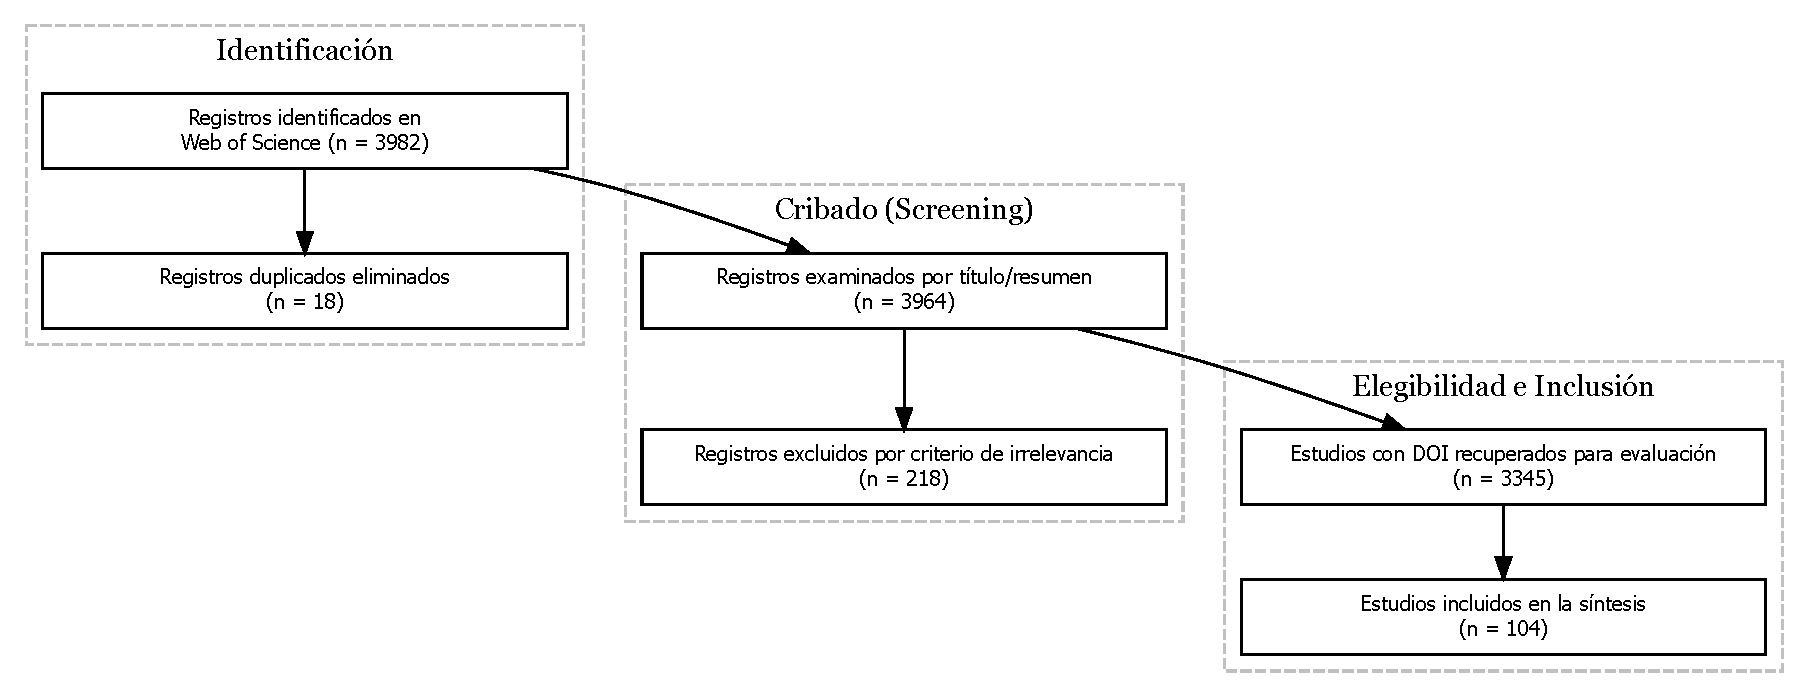
\includegraphics[width=1.0\textwidth]{../images/prisma-flowchart.pdf}
    \caption{Diagrama de Flujo Metodológico PRISMA 2020 para la selección de bibliografía de WoS.}
    \label{fig:prisma-flowchart}
\end{figure}